\documentclass[12pt]{beamer} %con pause
%\documentclass[12pt,handout]{beamer} %sin pause
%\documentclass[12pt,aspect=16:9]{beamer} %con pause, aspecto panorámico

\mode<presentation>{

%% La clase Beamer viene con varios temas de diapositiva predeterminados
%% que cambian los colores y diseños de las diapositivas. 
%\usetheme{Berlin}
%\usetheme{Boadilla}
%\usetheme{CambridgeUS}
\usetheme{Copenhagen}
%\usetheme{Goettingen}
%\usetheme{Hannover}
%\usetheme{Ilmenau}
%\usetheme{JuanLesPins}
%\usetheme{Luebeck}
%\usetheme{Madrid}
%\usetheme{Malmoe}
%\usetheme{Marburg}
%\usetheme{Montpellier}
%\usetheme{PaloAlto}
%\usetheme{Pittsburgh}
%\usetheme{Rochester}
%\usetheme{Singapore}
%\usetheme{Szeged}
%\usetheme{Warsaw}
%
%% Además, la clase Beamer tiene varios temas de color 
%% para cualquier tema de diapositiva
%\usecolortheme{beaver}
\usecolortheme{crane}
%\usecolortheme{dolphin}
%%\usecolortheme{lily}
%\usecolortheme{orchid}
%\usecolortheme{rose}
%\usecolortheme{seagull}
%\usecolortheme{seahorse}
%\usecolortheme{whale}
%%\usecolortheme{wolverine}
}

%---------------------------------------------------------------------------------------
%Mi configuración

\usepackage[utf8]{inputenc}
\usepackage[spanish]{babel}	%% manejos de idiomas
\usepackage[T1]{fontenc}
\usepackage{enumerate} %para listar y enumerar

\usepackage{ragged2e} %justificado y otras alineaciones
%%%\apptocmd{\frame}{}{\justifying}{} % Añade argumento opcional del frame

\usepackage{amsmath} %paquete matematico
\usepackage{amsthm} %para poner demostración a un teorema

\usepackage{graphicx} % paquete gráfico

\usepackage{chronosys} % lineas de tiempo

\uselanguage{spanish}
\languagepath{spanish}
\deftranslation[to=spanish]{Theorem}{Teorema}
\newtheorem{proposition}[theorem]{Proposición}

%----------------------------------------------------------------------------------------
%Propiedades del documento

\title[Elección y matemática]{La teoría de conjuntos ZF y el axioma de elección} 
%El título corto entre corchetes aparece en la parte inferior, 
%el título entre llaves solo aparece en la página de título
\author[Daniel Camarena]{Daniel Camarena Pérez} % Su nombre
\institute[UNI]{Universidad Nacional de Ingeniería} 
%Comportamiento similar al título
%\institute[UNI]{ 
%Universidad Nacional de Ingeniería \\ % Su institución para la página de título
%\medskip % espacio vertical medio
%\textit{vcamarenap@uni.pe} % su correo electrónico
%}
\logo{GEM}
\date{\today} % fecha, configure la traducción

%Mostrar contenido cada vez que inicia una nueva sección
\AtBeginSection[]
{
	\begin{frame}<beamer>{Contenido}
		\tableofcontents[currentsection,currentsubsection]
	\end{frame}
}
%----------------------------------------------------------------------------------------

\begin{document}

%----------------------------------------------------------------------------------------
%Inicio

\begin{frame}[plain] %plain limpia cabecera y pie de página
\titlepage 
% Imprime la página de título (title page) como el primer slide
\end{frame}

\begin{frame}[allowframebreaks]
\frametitle{Contenido} % Título del frame (slide)
\tableofcontents 
% Si usa los comandos \section{} y \subsection{}, automáticamente se cargan
\end{frame}

%----------------------------------------------------------------------------------------
%Desarrollo

%------------------------------------------------
\section{Conceptos Previos} 

%------------------------------------------------
\begin{frame}
\frametitle{Lógica matematica}

\textbf{Lógica de primer orden}: es un sistema formal diseñado para estudiar la inferencia en los lenguajes de primer orden. 

\textbf{Lenguaje de primer orden}: es un lenguaje formal (español), cuyos símbolos primitivos y reglas para unir esos símbolos están especificados con conectores lógicos, cuantificadores y funciones proposicionales. %\\~

\pause
\begin{itemize}
 \item Axioma: enunciado fundamental
 \item Concepto primitivo: concepto no definido
 \item Demostración: secuencia finita de enunciados que conducen de un conjunto de premisas a una sentencia dada
 \item Teorema: proposición derivada como la conclusión de una demostración
\end{itemize}
\end{frame}

\begin{frame}
\frametitle{Ejemplos}

 En la teoría de conjuntos ZF/ZFC:
\begin{itemize}
 \item Axioma: existe el conjunto vacío 
 \item Concepto primitivo: conjunto 
 \item Teorema: no existe el conjunto que es elemento de sí mismo 
\end{itemize}

\end{frame}

%------------------------------------------------

\begin{frame}
\frametitle{Ejemplo de demostración}

En la aritmética de Peano:
\begin{itemize}
 \item {\color{red} \textbf{Teorema}: Para todo $m$ y $n$ enteros positivos, si $m$ y $n$ son pares, entonces $m+n$ es par.}
 \item \textbf{Demostración}: Supongamos que $m$ y $n$ son enteros pares arbitrariamente elegidos. [Debe mostrarse que $m+n$ es par.]\\
  \begin{enumerate}[1.]
  	\item $m = 2r, n = 2s$ para algunos enteros $r$ y $s$ (por definición de par)
  	\item $m + n = 2r + 2s$ (por sustitución)
  	\item $m + n = 2(r + s)$ (mediante la factorización de $2$)
  	\item $r + s$ es un entero (pues es la suma de dos enteros)
  	\item $m + n$ es par (por definición de par)
  \end{enumerate}
\end{itemize}
\end{frame}

%------------------------------------------------

\begin{frame}
\frametitle{Teoría}

Sistema hipotético deductivo formado por un conjunto de proposiciones dentro de un lenguaje formal.\\

\pause
\begin{itemize}
 \item Consistente: si para cada par de fórmulas $(\varphi,\neg \varphi)$ solo una pertenece a la teoría
 \item Completa: si para cada par de fórmulas $(\varphi,\neg \varphi)$ al menos una pertenece a la teoría
\end{itemize}
\end{frame}

\begin{frame}
	\frametitle{Teoría}
			
\begin{center}
	¡¡En matemáticas todas las teorías son consistentes!!\\
	\dots\\
	Pero no todas son completas
\end{center}

\pause
Ejemplos:
\begin{itemize}
	\item La teoría de conjuntos ZFC 
	\item La teoría de la selección natural (no es teoría lógica, es científica)
\end{itemize}

\end{frame}

\begin{frame}
\frametitle{Paradoja}

Son argumentos donde
\begin{itemize}
 \item hay premisas no controvertidas y verdaderas.
 \item emplea un procedimiento no controversial.
 \item obtiene una conclusión
 \pause
 \begin{itemize}
  \item contradictoria
  \item absurda, inapropiada o inaceptable
 \end{itemize}
\end{itemize}

\vfill

\pause
Ejemplo: \href{https://es.wikipedia.org/wiki/Paradoja_de_Banach-Tarski}{La paradoja de Banach-Tarski}
\end{frame}

\section{Historia} 

%------------------------------------------------
\subsection{Antecedentes}

\begin{frame}
	\begin{alertblock}{}
		\justify
		La creación de la teoría de conjuntos se debe a una sola persona, Georg Cantor. Antes de ver ello, primero examinamos algunas contribuciones preliminares.
	\end{alertblock}
\end{frame}

\begin{frame}
\frametitle{Edad antigua y media}
La teoría de conjuntos tiene su origen en los razonamientos sobre el infinito, que datan desde la época griega.\\

\startchronology
[startyear=-500, stopyear=1650]
\chronoevent{-450}{Zenon} 
%
\chronoperiode{476}{1492}{Edad Media} 
\chronoevent{1638}{Galileo} 
\stopchronology
\end{frame}

\begin{frame}
\frametitle{Edad moderna}

El trabajo de Boole es el fundamento de la lógica informática.\\

\startchronology
[startyear=1840, stopyear=1880]
\chronoevent[textwidth=1.5cm]{1847}{Boole} 

\chronoevent[textwidth=1.5cm]{1851}{ ~~Bolzano } 

\chronoevent[]{1872}{Dedekind} 
\stopchronology

Dedekind publica su construcción formal de números reales y da una definición rigurosa de un entero.
\end{frame}

%------------------------------------------------
\subsection{La teoría ingenua de conjuntos.}

\begin{frame}
\frametitle{Georg Cantor}
\begin{figure}
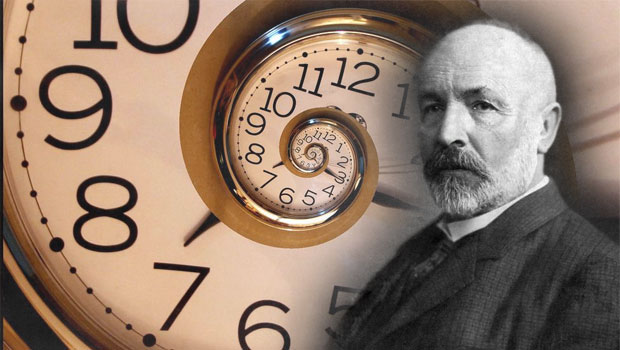
\includegraphics[width=1.\linewidth]{IMGS/cantor}
\end{figure}
\end{frame}

\begin{frame}
%\frametitle{Teoría de conjuntos de Cantor}

\justify
En 1874 Cantor publicó un artículo en el \textit{Crelle's Journal} ({\it \textcolor{blue}{Journal für die reine und angewandte Mathematik} }) 
el cual marca el nacimiento de la teoría de conjuntos.\\

\startchronology
[startyear=1870, stopyear=1910]
\chronoevent{1874}{Cantor} 
\chronoevent{1889}{Peano} 
\chronoperiode[startdate=false,stopdate=false,textwidth=3.5cm]{1897}{1902}{Paradojas;\endgraf 
1897: Burali-Forti;\endgraf
1899: Cantor;\endgraf
1901: Rusell} 
\stopchronology

\end{frame}

\begin{frame}
 \frametitle{La controversia}

\justify
Un segundo artículo fue presentado por Cantor en el \textit{Crelle's Journal} en 1878, pero la teoría de conjuntos ya se estaba convirtiendo en centro de la controversia. \\

Kronecker, quien estaba en la redacción de \textit{Crelle's Journal}, no estaba contento con las nuevas ideas revolucionarias contenidas en el documento de Cantor

\begin{block}{}
	\justify
	Cantor fue tentado a retirar el artículo, pero Dedekind persuadió a Cantor de no retirar su artículo y Weierstrass apoyó publicación.
\end{block}

\end{frame}

\begin{frame}
 \frametitle{El hotel de Hilbert}
  
 \begin{columns}[c] % La opción "c" especifica la alineación centrada vertical mientras la opción "t" es usada para alineación vertical superior

\column{.5\textwidth} % Columna izquierda con ancho ajustado al ancho de texto
\begin{figure}
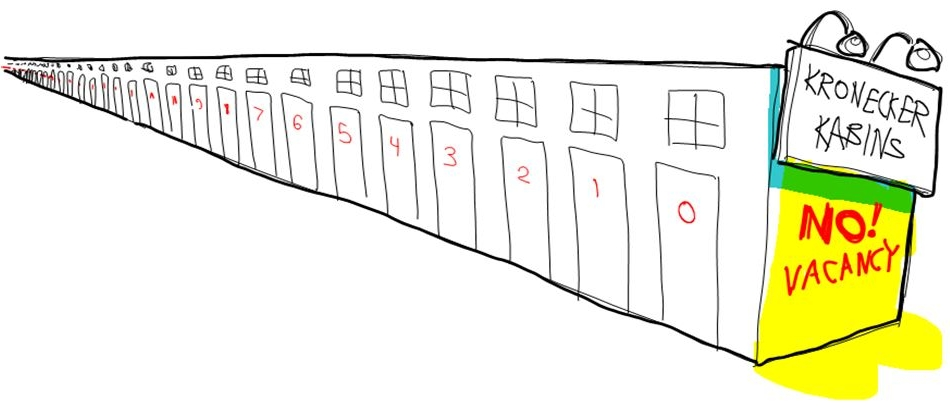
\includegraphics[width=1.1\linewidth]{IMGS/hilbert-hotel-L}
\end{figure}

\column{.5\textwidth} % Columna derecha con ancho ajustado al ancho de texto
\begin{figure}
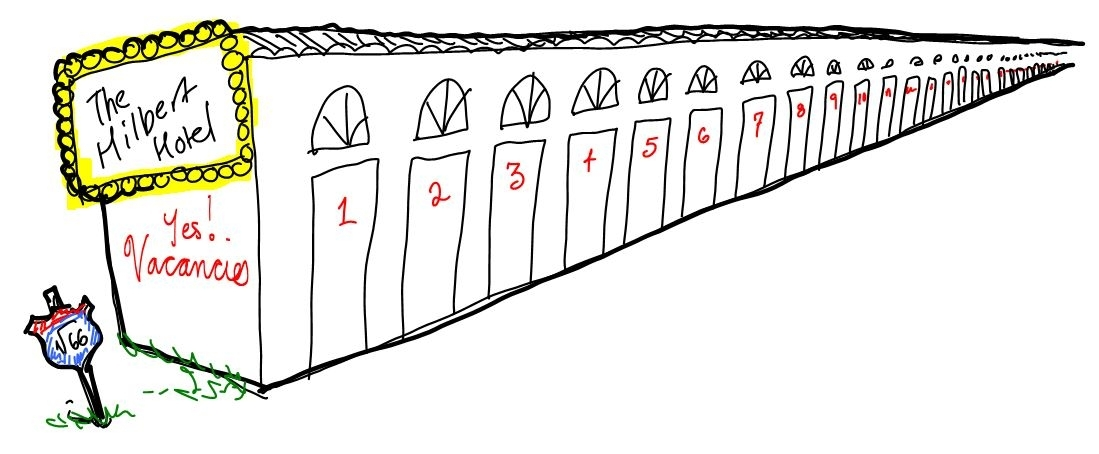
\includegraphics[width=1.1\linewidth]{IMGS/hilbert-hotel-R}
\end{figure}

\end{columns}

\vfill
\justifying
El hotel de Hilbert representa un acercamiento al entendimiento del infinito.
\end{frame}

\subsection{El discreto y el continuo}

\begin{frame}
 \frametitle{El conjunto de los números naturales}

\justify
Peano, en 1889, publica \textit{Arithmetices principia, nova methodo exposita} que donde expone los axiomas de Peano\\
 
\begin{block}{Axiomas de Peano}
 Existe un conjunto $N$, no vacío, y una función $s:N \to N$ de modo que se cumplen las siguientes propiedades:
 
 \pause
 \begin{enumerate}
  \item $s$ es inyectiva.
  \item $N\setminus s(N) = \{1\}$ %es un conjunto unitario, dicho elemento se denota $1$.
  \item Todo subconjunto de $N$ que contiene al $1$ y tiene la propiedad, $\forall n\in X, s(n)\in N$, no es otro sino $N$.
 \end{enumerate}
 \end{block}
\end{frame}

\begin{frame}
 \frametitle{El todo no es mayor que las partes}

\justify
Ya se tiene que $N$ es un modelo del conjunto de números naturales $\mathbb{N}$. En este modelo,
\begin{theorem}[Infinitud]
 Todo conjunto infinito tiene un subconjunto propio que se puede poner en correspondencia uno-uno a si mismo.
\end{theorem}

\pause
Es decir, todo conjunto infinito tiene una parte equipotente a si mismo.
\end{frame}

\begin{frame}
 \frametitle{El continuo}
 Dedekind logró construir los números reales ($\mathbb{R}$) a partir de los números racionales ($\mathbb{Q}$) usando la técnica de las \textit{cortaduras de Dedekind}.\\
 
 \pause
 {\color{red} Una pregunta que surge es si el infinito de los naturales y el infinito de los reales son iguales.}
 
 \pause
 \begin{theorem}[El continuo]
  No existe una biyección entre el conjunto de los naturales y el conjunto de los reales.
 \end{theorem}
\end{frame}


\begin{frame}
 \frametitle{La hipótesis del continuo}
 
 \begin{theorem}
  La potencia de un conjunto no es equipotente al conjunto.
 \end{theorem} 
 
 \pause
 \begin{theorem}
  El continuo es equipotente de a la potencia del discreto, es decir, 
  $$ \mathrm{card}\left( \mathbb{R} \right) = \mathrm{card} \left( P(\mathbb{N}) \right)$$
 \end{theorem}
 
 \pause
 \begin{alertblock}{Hipótesis del Continuo (HC)}
  Todo subconjunto infinito de $\mathbb{R}$ es o bien equipotente a $\mathbb{N}$ o bien equipotente a $\mathbb{R}$.
 \end{alertblock}
\end{frame}


%------------------------------------------------
\subsection{La paradoja del barbero}

\begin{frame}
 \frametitle{La paradoja del barbero}
 
 \begin{figure}
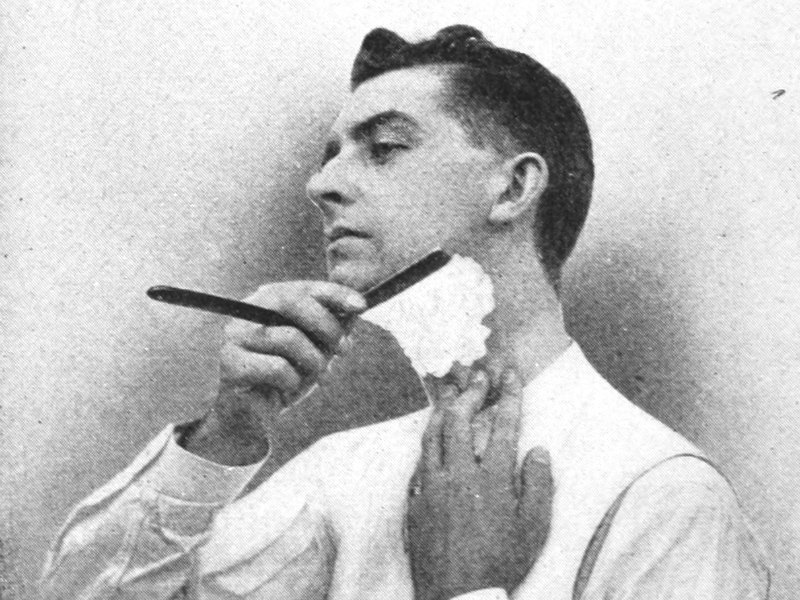
\includegraphics[width=0.8\linewidth]{IMGS/barbero}
\end{figure}
\end{frame}

\begin{frame}
 \frametitle{La paradoja de barbero}
 
\begin{block}{}
	Definamos un conjunto
	$$
	A = \{ X | ~X \text{no es elemento de} ~X\}
	$$
	Russell entonces se preguntó: 
	¿Es $A$ un elemento de $A$?
\end{block}

\pause
Tanto el supuesto de que $A$ es un miembro de $A$ y que $A$ no es un miembro de $A$ conllevan a una contradicción. 

\pause
\begin{center}
 ¡La propia construcción del conjunto parece dar una paradoja!
\end{center}
\end{frame}


\section{La teoría de conjuntos ZFC}

%------------------------------------------------
\subsection{Una nueva teoría de conjuntos}

\begin{frame}
\frametitle{Ernst Zermelo}
\begin{figure}
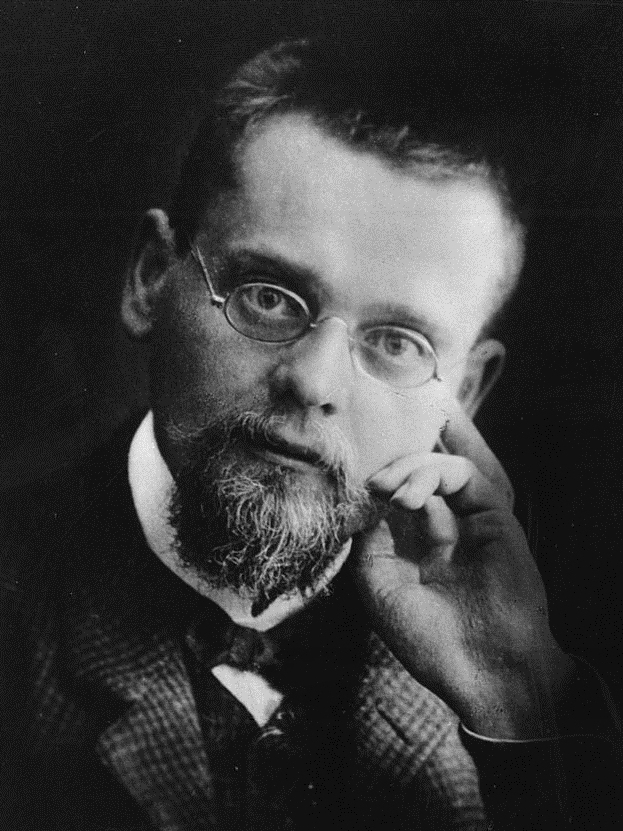
\includegraphics[width=0.5\linewidth]{IMGS/zermelo}
\end{figure}
\end{frame}

%------------------------------------------------

\begin{frame}
\frametitle{Una nueva teoría de conjuntos}

\startchronology
[startyear=1902, stopyear=1928]
%color=black, height=5ex, with=\hsize]
\chronoperiode[startdate=false,stopdate=false,textwidth=3.2cm]{1904}{1908}{\qquad Zermelo;\endgraf 
1904: Buen orden;\endgraf
1908: Axiomas Z} 
%%1er artículo de teoría de conjuntos. Él describe rigurosamente la noción de infinito. Muestra que los infinitos vienen en diferentes tamaños. Prueba el polémico resultado de que casi todos los números son trascendentales.
\chronoperiode[textwidth=2.8cm]{1910}{1919}{\qquad Russell\endgraf
\quad Whitehead}
\chronoevent[textwidth=2.cm]{1922}{~~Axiomas\endgraf
\qquad ZF}
\chronoevent[textwidth=1.5cm]{1926}{\quad Banach-Tarski} 
\stopchronology

\end{frame}


\begin{frame}
 \frametitle{Los axiomas Zermelo-Fraenkel}

\begin{enumerate}
	\item[I]	Extensionalidad: igualdad de conjuntos
	\item[II]	Vacío: existe al menos un conjunto
	\item[III]  Unión: unión de conjuntos
	\item[IV]	Potencia: el conjunto de los subconjuntos
	\item[V]	Infinitud: existe un conjunto infinito
	\item[VI]	Reemplazamiento %fórmulas y evaluaciones
	\item[VII]	Relación de Tipos %implica el ax especificacion
	\item[AC]	Elección%: para cualquier familia de conjuntos el producto cartesiano es no vacío
\end{enumerate}
\end{frame}

\begin{frame}
 \frametitle{Resolviendo la paradoja de Rusell}

\textbf{Axioma del Esquema de Comprensión (FALSO)}. Si $P$ es una propiedad, entonces existe un conjunto $Y = \{x: P(x)\}$.\\~

\pause
Y el conjunto de todos los conjuntos no existe, en todo caso: 
\begin{center}
 ¡¡ es el concepto del conjunto de todos los conjuntos lo que es paradójico, no la idea misma de la comprensión de un conjunto !!
\end{center}
\end{frame}

\begin{frame}
 \frametitle{El Buen Orden}
 
\justify
Todo subconjunto de los números naturales se puede ordenar en el sentido intuitivo.\\

\pause
El concepto del buen orden generaliza la propiedad de buen orden de los naturales y da origen a la teoría de los números ordinales.
 
\pause
\begin{block}{Principio del Buen Orden}
  Todo subconjunto, no vacío, de naturales admite un primer elemento.
\end{block}
\end{frame}

\begin{frame}
 \frametitle{El Buen Orden}

\justify
La noción de orden abstracta se define apelando a la noción de subcojunto.\\

\pause
 \begin{theorem}[Teorema del Buen Orden]
  Todo subconjunto no vacío de naturales admite un primer elemento.
 \end{theorem}
 
 \pause
 \begin{proof}
  \begin{center}
  ¡¡Requiere hacer uso de un axioma adicional, el Axioma de Elección!!
  \end{center}
 \end{proof}
\end{frame}

\subsection{El Axioma de Elección}

\begin{frame}
 \frametitle{El Axioma de Elección}
 
 \begin{figure}
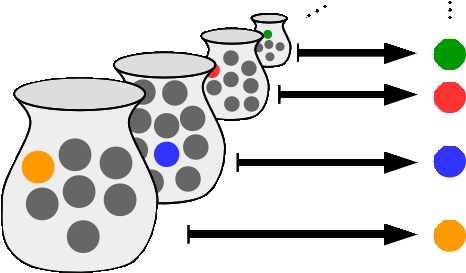
\includegraphics[width=0.7\linewidth]{IMGS/choice}
\end{figure}
\end{frame}
  
 \begin{frame}
 \frametitle{La paradoja de Banach-Tarski}
 
 \begin{theorem}
  Es posible dividir una esfera de radio $1$ en ocho partes disjuntas dos a dos, de modo que, aplicando movimientos oportunos a cinco de ellas, obtengamos 
  nuevos conjuntos que constituyan una partición de una esfera de radio $1$, y lo mismo ocurra con las tres partes restantes.
 \end{theorem}
\end{frame}

\begin{frame}
 \frametitle{La paradoja de Banach-Tarski}
 
 \begin{figure}
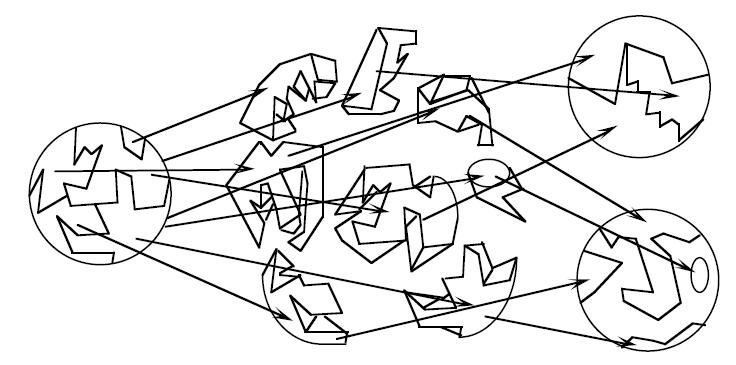
\includegraphics[width=1.\linewidth]{IMGS/tarski}
\end{figure}
\end{frame}

%------------------------------------------------
\subsection{Consistencia y completitud de la teoría ZFC}

\begin{frame}
\frametitle{Godel y Cohen}

\begin{columns}[c]

\column{.5\textwidth} 
\begin{figure}
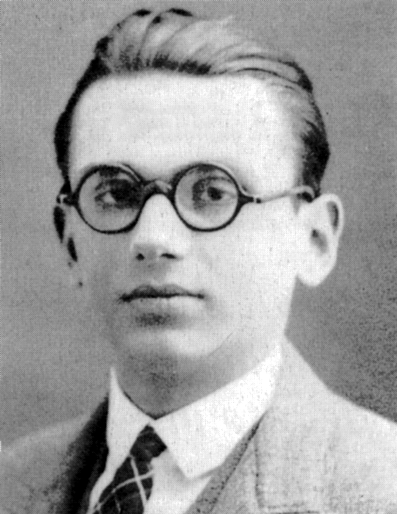
\includegraphics[width=0.7\linewidth]{IMGS/godel}
\end{figure}

\column{.5\textwidth} 
\begin{figure}
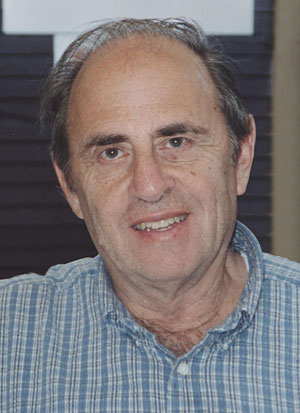
\includegraphics[width=0.7\linewidth]{IMGS/cohen}
\end{figure}

\end{columns}
\end{frame}

%------------------------------------------------

\begin{frame}
\frametitle{Goedel y Cohen}

\startchronology
[startyear=1930, stopyear=1965]
\chronoevent[textwidth=1.8cm]{1931}{ ~~Goedel\endgraf
Incompletitud} 
\chronoperiode[startdate=false]{1934}{1935}{~~Zorn}
\chronoevent[textwidth=1.5cm]{1940}{\quad Goedel\endgraf
Consistencia}
\chronoevent[textwidth=1.5cm]{1963}{\quad Cohen}
\stopchronology

\end{frame}

%------------------------------------------------

\begin{frame}
 \frametitle{Equivalencias al Axioma de Elección}
 
 \begin{itemize}
  \item Principio Multiplicativo
  \item Principio de Buen Orden
  \item El Lema de Zorn
  \item Principio de Kuratowski
 \end{itemize}
\end{frame}

\begin{frame}
 \frametitle{Aplicaciones del Axioma de Elección}
 
 \begin{itemize}
  \item Todo espacio vectorial tiene una base (Álgebra Lineal).
  \item La unión enumerable de conjuntos enumerables es enumerable.
  \item Existe un conjunto de números reales que no es Lebesgue-medible (Teoría de la Medida).
  \item El producto de espacios compactos es compacto (Topología).
  \item Todo anillo con unidad tiene un ideal maximal (Álgebra).
  \item Todo orden parcial puede extenderse a un orden total.
  \item El teorema de Hahn-Banach (Análisis Funcional).
  \item El teorema de completud para la lógica de primer orden.
  \item Toda álgebra de Boole es isomorfa a un campo de conjuntos.
 \end{itemize}
\end{frame}

\begin{frame}
 \frametitle{El axioma de elección (AC) y ZF}
 
 \begin{theorem}
  Bajo la teoría ZF, el axioma de elección es equivalente a la hipótesis del continuo generalizado.
 \end{theorem}
 
 \pause
 \begin{theorem}[Indecibilidad; \cite{godel1938consistency}]
  El axioma de elección y la hipótesis del continuo generalizado es consistente de los axiomas de la teoría de conjuntos ZF.
 \end{theorem}
 %no puede refutarse con ZF
 
 \pause
 \begin{theorem}[Independencia; \cite{cohen2008set}]
  El axioma de elección y la hipótesis del continuo generalizado es independiente de los axiomas de la teoría de conjuntos ZF.
 \end{theorem}
 %no puede probarse con ZF
\end{frame}


\begin{frame}
\frametitle{Una teoría de conjuntos estándar}

\begin{alertblock}{Teoría ZFC}
	\justify
	La teoría de conjuntos es uno de los mayores logros de la matemática moderna. Básicamente todos los conceptos matemáticos, métodos y resultados admiten la representación dentro de la teoría axiomática de conjuntos.
\end{alertblock}

%Forzamos citaciones fantasmas
\nocite{jech2003set,kuratowski2014introduction,pickover2009math,herrlich2006axiom}.
\end{frame}
%----------------------------------------------------------------------------------------

%----------------------------------------------------------------------------------------
%Cierre

\begin{frame}[allowframebreaks]
\frametitle{Referencias}
\bibliographystyle{plain}
\bibliography{bibliografia}
\end{frame}

\begin{frame}
\centering {\bfseries\Huge ¡Muchas Gracias!}
\end{frame}
%----------------------------------------------------------------------------------------

\end{document}
